After the assembly inspection has performed the static analysis and flagged programs with potential timing vulnerabilities, OptiFuzz tries and confirm their presence. 
For this, we have created a fuzzer.
First, the fuzzer compiles the program with the specified compiler and optimization level flags.
Then, the fuzzer runs the program with random inputs and measures the execution time.

The process goes as follows: 
First, the fuzzer itself is compiled into object files that are not yet linked. 
This compilation only needs to happen once. 
Then, each of the programs flagged by the static assembly analysis is compiled with the specified compiler and linked with the pre-compiled fuzzer. 
This step is carried out for each of the supplied optimization flags such that the program is fuzzed on all supplied optimization levels.

Then, for each linked program, the fuzzer generates inputs according to 'input classes' which are explained later in this section. 
For each input, the fuzzer chooses a uniformly random class among the supplied ones. 
This way there is no biased order in which the inputs from different classes are used, and thus potential noise is likely to affect all classes equally. 
This is important when comparing timing distributions in the following statistical analysis. 

\begin{figure}[H]
    \centering
    \tikzstyle{box-nb} = [rectangle, minimum width=1.3cm, minimum height=0.3cm, text centered]
\tikzstyle{box} = [rectangle, minimum width=2.2cm, minimum height=0.8cm, text centered, draw=black]
\tikzstyle{arrow} = [thick,->,>=stealth]

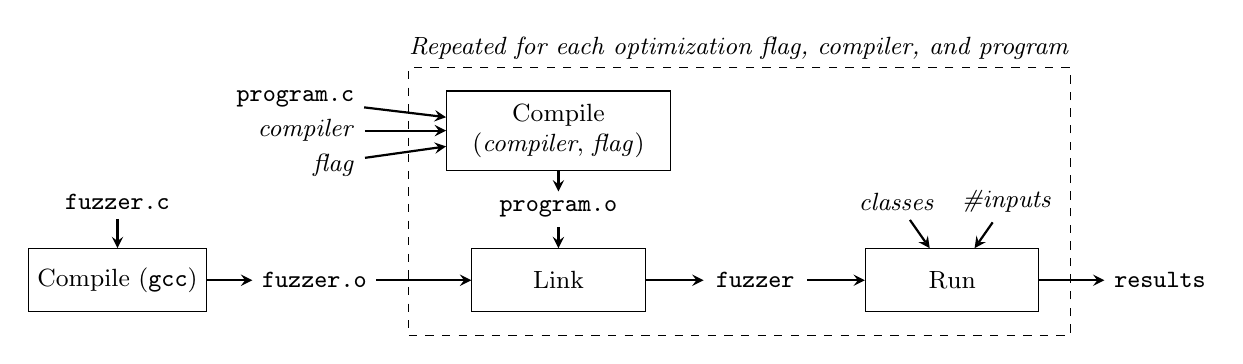
\begin{tikzpicture}
  \node (comp_prog) [box] {\small \begin{tabular}{c} Compile \\ (\textit{compiler}, \textit{flag}) \end{tabular} };
  \node (programo) [box-nb, below of=comp_prog] {\small \texttt{program.o}};
  \node (link) [box, below of=programo, yshift=0.1cm] {\small Link};
  \node (fuzzero) [box-nb, left of=link, xshift=-2.1cm] {\small \texttt{fuzzer.o}};
  \node (comp_fuzz) [box, left of=fuzzero, xshift=-1.5cm] {\small Compile (\texttt{gcc})};
  \node (fuzzerc) [box-nb, above of=comp_fuzz] {\small \texttt{fuzzer.c}};
  \node (fuzzer) [box-nb, right of=link, xshift=1.5cm] {\small \texttt{fuzzer}};
  \node (run) [box, right of=fuzzer, xshift=1.5cm] {\small Run};
  \node (classes) [box-nb, above of=run, xshift=-0.7cm] {\small \textit{classes}};
  \node (inputs) [box-nb, above of=run, xshift=0.7cm] {\small \textit{\#inputs}};
  \node (results) [box-nb, right of=run, xshift=1.64cm] {\small \texttt{results}};
  \node (programc) [box-nb, left of=comp_prog, yshift=0.4cm, xshift=-2.34cm] {\small \texttt{program.c}};
  \node (compiler) [box-nb, left of=comp_prog, xshift=-2.2cm] {\small \textit{compiler}};
  \node (flag) [box-nb, left of=comp_prog, yshift=-0.4cm, xshift=-2.13cm, yshift=-0.04cm] {\small \textit{\quad\ \ flag}};
  \node (repeat) [rectangle, draw=black, dashed, minimum height=3.4cm, minimum width=8.4cm, yshift=-0.9cm, xshift=2.3cm] {};
  \node (repeat-text) [box-nb, above of=repeat, yshift=0.95cm] {\small \textit{Repeated for each optimization flag, compiler, and program }};
  
  \draw [arrow] (fuzzerc) -- (comp_fuzz);
  \draw [arrow] (comp_fuzz) -- (fuzzero);
  \draw [arrow] (comp_prog) -- (programo);
  \draw [arrow] (programo) -- (link);
  \draw [arrow] (fuzzero) -- (link);
  \draw [arrow] (link) -- (fuzzer);
  \draw [arrow] (fuzzer) -- (run);
  \draw [arrow] (run) -- (results);
  \draw [arrow] (programc)-- (comp_prog);
  \draw [arrow] (compiler) -- (comp_prog);
  \draw [arrow] (flag) -- (comp_prog);
  \draw [arrow] (classes) -- (run);
  \draw [arrow] (inputs) -- (run);
\end{tikzpicture}
    \caption{Illustration of the process of compiling and fuzzing programs.}
    \label{fig:fuzzer-pipeline}
  \end{figure}

The fuzzer then runs through all the generated inputs and calls the internally linked program with each of them. 
The program's execution time is measured every time it is run. 
The fuzzer repeats the run-through multiple times (50) to allow for the detection of outliers and get as precise results as possible. 
Note that a run-through consists of fuzzing with all randomly generated inputs.
Hence, some specific input is not repeated before all other inputs have been run again. 
This ensures that any noise that results in longer execution times is spread out over all (or many) of the inputs. 
This minimizes the chance of falsely identifying an input or fuzzing class as the cause of longer execution times.

We use different input classes for the inputs to the fuzzer, instead of always generating completely random numbers. 
This is done to try and capture variable execution time that only takes place in a small sample of the values. 
As an example, a program might have a timing leak only if one of the inputs is zero. 
If we only used uniformly random 64-bit numbers it would be unlikely that we would identify a vulnerability like that. 
Hence, the need for input classes. 
As mentioned in Section \ref{sec:code-generation}, for each program, there are an $x$ and a $y$ value. 
All input classes generate inputs concerning these inputs can be seen in the following list.
\begin{itemize}
    \setlength\itemsep{-0.5em}
    \item \texttt{UNIFORM}: $x$ and $y$ are uniformly random 64-bit numbers.
    \item \texttt{EQUAL}:  $x$ and $y$ are the same uniformly random 64-bit number.
    \item \texttt{MAX64}: Either $x$ or $y$ is a random 64-bit number, the other is uniformly random.
    \item \texttt{XZERO}: $x$ is 0, $y$ is a uniformly random number.
    \item \texttt{YZERO}: $y$ is 0, $x$ is a uniformly random number.
    \item \texttt{XLTY}: Two uniformly random numbers are generated, $x$ is set to the smaller, $y$ to the larger.
    \item \texttt{YLTX}: Two uniformly random numbers are generated, $y$ is set to the smaller, $x$ to the larger.
    \item \texttt{SMALL}: $x$ and $y$ are uniformly random 8-bit numbers (the upper 56 bits are set to 0).
    \item \texttt{FIXED}: $x$ and $y$ have the same fixed number $0x12345678$ (used for Welsh's t-test).
\end{itemize}
These classes have been made based on observations of values commonly used in comparisons in emitted assembly code.

Precise measurements of a program's execution time are not trivial to perform. 
Measurements can be influenced by several things including context switches, interrupts, out-of-order execution, varying CPU clock speed, and congestion. 
After researching our options, we ended up using the Time Stamp Counter (\texttt{TSC}) which is a high-resolution counter that (on newer machines) increases at a fixed rate independent of processor frequency. 
This method is heavily inspired by the suggestions and results from an Intel white paper \citep{intel-benchmark-code-execution}.
Using the \texttt{TSC} as a reference for time is the most efficient way of fetching wall time and with respect to the efficiency the best approach.
This method is the one suggested by \citep{intel-benchmark-code-execution} and is the one used in the DudeCT black-box testing tool by \citep{dudect}.
Alternatives like \texttt{HPET} with higher resolutions exist but which reads the time from a platform resource instead of a register, making it much slower \citep[b]{intel-reference}.
This approach also allowed us to avoid the timings being skewed by the CPU performing out-of-order execution.
Out-of-order executions could lead to the instructions being reordered resulting in not reading the \texttt{TSC} (with the \texttt{RDTSC}(\texttt{P}) instruction) at the exact time we want to. 
This is done by utilizing the non-privileged \texttt{CPUID} instructions serializing capabilities that ensure that memory transactions for previous instructions are completed before the next instruction is executed \citep[a]{intel-reference}.

Later, when using these results in the analysis, we use the minimum time for all executions with the same input.
Using the minimum time as the true execution time instead of the mean filters out the noise from outliers that are the results of i.e. context-switches or congestion \citep{robust-benchmarking}. 
In comparison to DudeCT from \citep{dudect}, which just removes the top 5\% of the longest measured execution times to reduce such noise, our approach is not prone to accidentally removing measurements of large execution times that are correct and not the result of noise.

\subsubsection{Limitations}
We consider the fuzzer successful when it can consistently measure clear differences in the execution time of a program with respect to its inputs. 
The time difference makes it possible to make an educated guess on what the given inputs look like and hence opens up a potential timing-based side-channel attack. 
This does indeed indicate that the program is vulnerable.

If, on the other hand, the results of this analysis fail to indicate obvious timing differences, then it is not safe to assume that it is then constant time. 
Since the fuzzer is conservative, it under-approximates what programs are vulnerable to timing attacks.
Hence, a limitation is that the input classes used are not necessarily able to capture an event causing variable-time behavior of a program. 

Furthermore, even with the actions taken to get as precise timings as possible, the analysis is still prone to some noise. 
Specifically, it is worth noting that when running this in user-land the fuzzer could be influenced by interrupts and preemption (being context switches triggered by the OS instead of the process yielding). 
To disable interrupts and preemption, one is required to run the code in kernel space, which is a possible future extension of the fuzzer. 
However, as a compromise, the fuzzer can be run with higher priority to reduce some noise. 
